\documentclass[tikz,border=4pt]{standalone}
\usetikzlibrary{arrows.meta}
\begin{document}
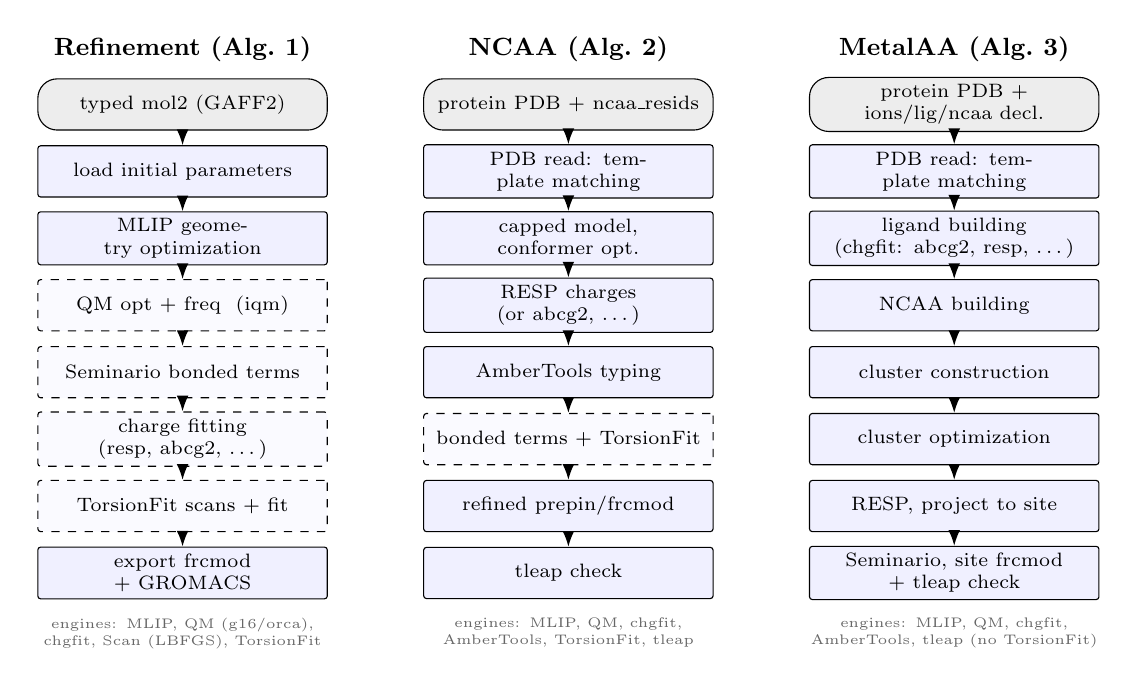
\begin{tikzpicture}[
  stage/.style={draw, rounded corners=1pt, fill=blue!6, font=\scriptsize, align=center,
                inner sep=2.5pt, text width=3.5cm, minimum height=6.5mm},
  opt/.style={stage, dashed, fill=blue!2},
  io/.style={draw, rounded corners=7pt, fill=gray!14, font=\scriptsize, align=center,
             inner sep=2.5pt, text width=3.5cm, minimum height=6.5mm},
  arr/.style={-{Latex[length=2mm]}, semithick},
  colhead/.style={font=\small\bfseries},
  engines/.style={font=\tiny, text=black!60, align=center, text width=3.7cm}]

% ---------- Refinement ----------
\node[colhead]                       (m-h) at (0, 12.4) {Refinement (Alg.~1)};
\node[io]                            (m-in) at (0, 11.7) {typed mol2 (GAFF2)};
\node[stage]                         (m-p0) at (0, 10.85) {load initial parameters};
\node[stage]                         (m-p1) at (0, 10.0) {MLIP geometry optimization};
\node[opt]                           (m-p2) at (0, 9.15) {QM opt $+$ freq \ (iqm)};
\node[opt]                           (m-p3) at (0, 8.3) {Seminario bonded terms};
\node[opt]                           (m-p4) at (0, 7.45) {charge fitting\\(resp, abcg2, \dots)};
\node[opt]                           (m-p5) at (0, 6.6) {TorsionFit scans $+$ fit};
\node[stage]                         (m-p6) at (0, 5.75) {export frcmod $+$ GROMACS};
\node[engines, anchor=north]         (m-e) at (0, 5.3) {engines: MLIP, QM (g16/orca), chgfit, Scan (LBFGS), TorsionFit};

% ---------- NCAA ----------
\node[colhead]                       (n-h) at (4.9, 12.4) {NCAA (Alg.~2)};
\node[io]                            (n-in) at (4.9, 11.7) {protein PDB $+$ ncaa\_resids};
\node[stage]                         (n-p0) at (4.9, 10.85) {PDB read: template matching};
\node[stage]                         (n-p1) at (4.9, 10.0) {capped model, conformer opt.};
\node[stage]                         (n-p2) at (4.9, 9.15) {RESP charges\\(or abcg2, \dots)};
\node[stage]                         (n-p3) at (4.9, 8.3) {AmberTools typing};
\node[opt]                           (n-p4) at (4.9, 7.45) {bonded terms $+$ TorsionFit};
\node[stage]                         (n-p5) at (4.9, 6.6) {refined prepin/frcmod};
\node[stage]                         (n-p6) at (4.9, 5.75) {tleap check};
\node[engines, anchor=north]         (n-e) at (4.9, 5.3) {engines: MLIP, QM, chgfit, AmberTools, TorsionFit, tleap};

% ---------- MetalAA ----------
\node[colhead]                       (k-h) at (9.8, 12.4) {MetalAA (Alg.~3)};
\node[io]                            (k-in) at (9.8, 11.7) {protein PDB $+$ ions/lig/ncaa decl.};
\node[stage]                         (k-p0) at (9.8, 10.85) {PDB read: template matching};
\node[stage]                         (k-p1) at (9.8, 10.0) {ligand building\\(chgfit: abcg2, resp, \dots)};
\node[stage]                         (k-p2) at (9.8, 9.15) {NCAA building};
\node[stage]                         (k-p3) at (9.8, 8.3) {cluster construction};
\node[stage]                         (k-p4) at (9.8, 7.45) {cluster optimization};
\node[stage]                         (k-p5) at (9.8, 6.6) {RESP, project to site};
\node[stage]                         (k-p6) at (9.8, 5.75) {Seminario, site frcmod\\$+$ tleap check};
\node[engines, anchor=north]         (k-e) at (9.8, 5.3) {engines: MLIP, QM, chgfit, AmberTools, tleap (no TorsionFit)};

\foreach \c in {m,n,k} {
  \foreach \i/\j in {in/p0, p0/p1, p1/p2, p2/p3, p3/p4, p4/p5, p5/p6} {
    \draw[arr] (\c-\i) -- (\c-\j);
  }
}
\end{tikzpicture}
\end{document}
